\section{Teplotní senzory}

\begin{figure}[H]
\centering
\begin{subfigure}{.5\textwidth}
    \centering
    \input{images/svg/otopna-soustava/vyrez-teplotni-senzory-krb.pdf_tex}
    \caption{Teplotní senzor na kouřovodu krbu.}
    \label{fig:vyrez-teplotni-senzory-krb}
\end{subfigure}%
\begin{subfigure}{.5\textwidth}
   	\centering
   	\input{images/svg/otopna-soustava/vyrez-teplotni-senzory-zasobnik-otopne-vody.pdf_tex}
     \caption{Teplotní senzory v zásobníku otopné vody.}
    \label{fig:vyrez-teplotni-senzory-zasobnik-otopne-vody}
\end{subfigure}%
\caption[Umístění teplotních senzorů.]{Výřez z obrázku \ref{fig:otopna-soustava-a-elektronika-rez-domu}. Umístění teplotních senzorů.}
\end{figure}

Na obrázku \ref{fig:vyrez-teplotni-senzory-krb} je výřez části z celkového nákresu (obrázek \ref{fig:otopna-soustava-a-elektronika-rez-domu}) systému znázorňující umístění teplotního senzoru u kouřovodu krbu. Pro snímání teploty z kouřovodů u krbů slouží termočlánek typu K od výrobce Guenther. Teplotní rozsah je od -100 °C do 400 °C, takže je dostatečná teplotní rezerva. Průměr kovové ochranné trubičky je 4 mm s délkou 60 mm. Přívodní kabel je dlouhý 3 m se skelným opletením. Termočlánek je zobrazen na obrázku \ref{fig:termoclanek-72-21301041-k}.

\begin{figure}[H]
    \centering
    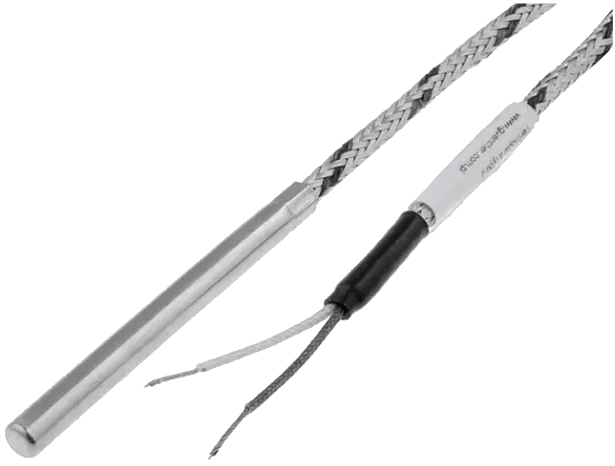
\includegraphics[width=0.4\textwidth]{images/termoclanek-72-21301041-k.png}
    \caption[Termočlánek 72-21301041 typu K.]{Termočlánek 72-21301041 typu K \cite{termoclanek-k}.}
    \label{fig:termoclanek-72-21301041-k}
\end{figure}

Na obrázku \ref{fig:vyrez-teplotni-senzory-zasobnik-otopne-vody} je výřez části z celkového nákresu (obrázek \ref{fig:otopna-soustava-a-elektronika-rez-domu}) systému znázorňující umístění teplotních senzorů v zásobníku otopné vody. Pro snímání teplot z centrálního zásobníku otopné vody, venkovní teploty a~prostorových teplot z jednotlivých místností slouží teplotní senzor DS18B20 od výrobce Maxim. Umožňuje měřit v teplotním rozsahu od -55 °C do +125~°C. V~rozsahu od -10 °C do +85 °C měří s přesností ±0,5 °C. Senzor umožňuje měřit teplotu s přesností 12 bitů. Pro komunikaci využívá 1-Wire sběrnici (způsob komunikace je popsán v \ref{sec:1-wire-sbernice} v části 1-Wire sběrnice). Ve svém konkrétním řešením využívám senzory v pouzdře TO-92 pro nástěnné snímače prostorové teploty, pro centrální zásobník otopné vody a~venkovní teplotu je senzor uložen do ochranného pouzdra.

\subsection{Realizace 1-Wire sběrnice u zásobníku otopné vody}
\begin{figure}[H]
   \centering
   \def\svgwidth{0.2\columnwidth}
   \input{images/svg/otopna-soustava/vyrez-1-wire-sbernice-u-zasobniku-otopne-vody.pdf_tex}
   \caption[Umístění sdružení 1-Wire sběrnice u zásobníku otopné vody.]{Výřez z obrázku \ref{fig:otopna-soustava-a-elektronika-rez-domu}. Umístění sdružení 1-Wire sběrnice u zásobníku otopné vody.}
    \label{fig:vyrez-1-wire-sbernice-u-zasobniku-otopne-vody}
\end{figure}

Na obrázku \ref{fig:vyrez-1-wire-sbernice-u-zasobniku-otopne-vody} je výřez části z celkového nákresu (obrázek \ref{fig:otopna-soustava-a-elektronika-rez-domu}) systému znázorňující umístění spojení 1-Wire sběrnice u zásobníku otopné vody. Na obrázku \ref{fig:dps-1-wire-sbernice-u-zasobniku-otopne-vody} je realizovaná DPS pro teplotní senzory u zásobníku otopné vody. Princip zapojení včetně ochrana na napájecí i datové části je popsán v~části \ref{sec:dps-se-vstupy-vystupy-pro-raspberry-pi} (datová část 1-Wire sběrnice). Na obrázku \ref{fig:instalacni-krabice-cidla-u-zasobniku-otopne-vody} je vidět horní část DPS vložená do instalační krabice. Celkově je zde k dispozici 6~pozic pro upevnění přes svorkovnice teplotní senzory. V současnosti jsou zde napojeny 3 teplotní senzory pro snímání teplot z horní, střední a~spodní části zásobníku otopné vody. Umístění senzorů je dáno výrobcem zásobníku a senzory jsou vloženy do dutiny. Samotná 1-Wire sběrnice je realizovaná pomocí UTP kabelu kategorie 5e. Na pinu číslo 4 jsou DATA, na pinu 5 je zem (GND) a na pinu 3 je napájení 5~V. Pro měření venkovní teploty je senzor DS18B20 v~pouzdře TO-92 připevněn na UTP kabel a zataven plastovou hmotou, na níž je následně nanesena smršťovací ochranná bužírka. Na obrázku \ref{fig:zasobnik-otopné-vody} jsou vyznačená místa s~umístěním teplotních senzorů. Celkové schéma zapojení je v příloze \ref{app:schemata-ostatni}.

\begin{figure}[H]
\centering
\begin{subfigure}{.5\textwidth}
    \centering
    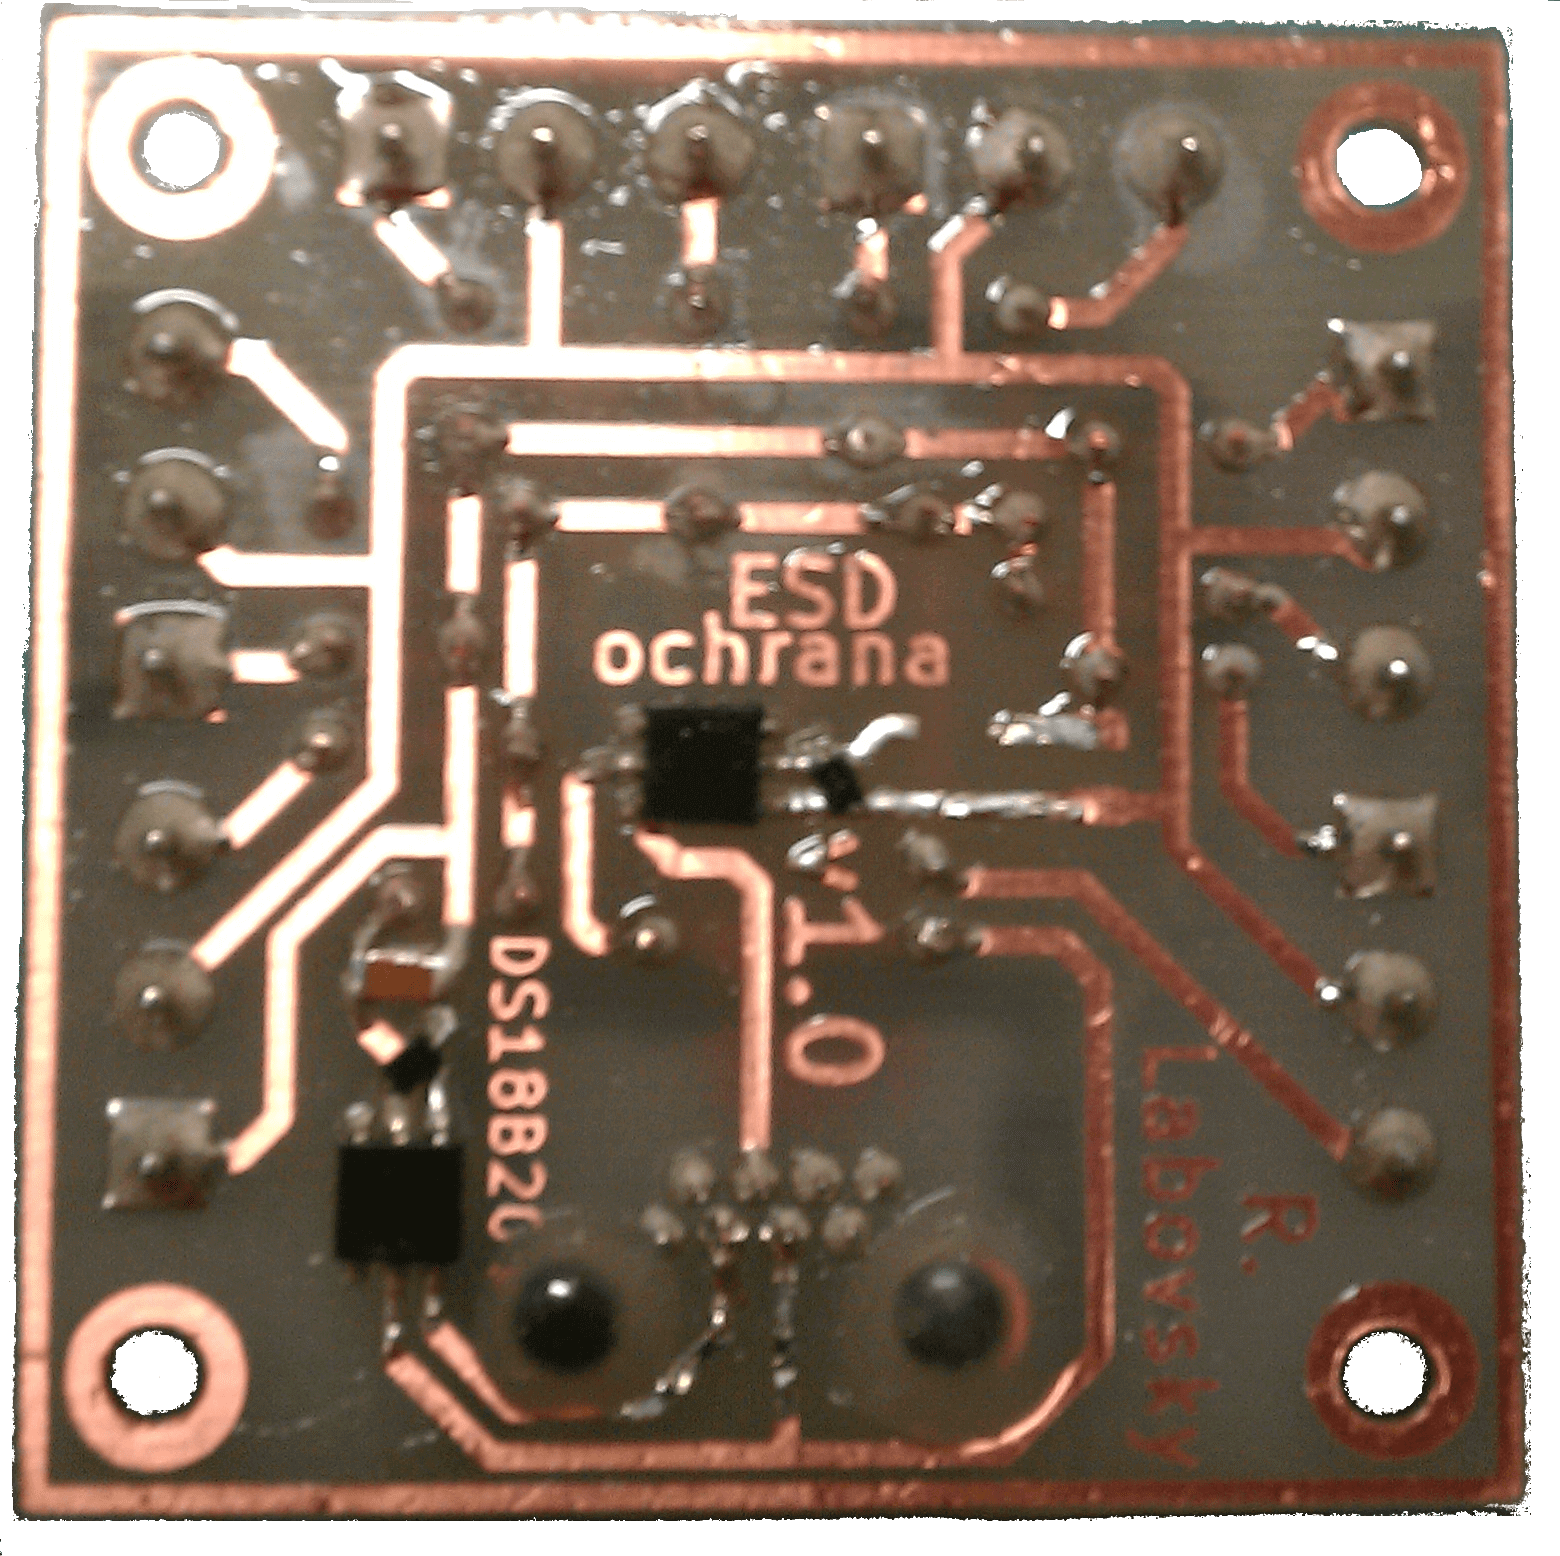
\includegraphics[width=\textwidth]{images/zasobnik-otopne-vody/dps-1-wire-sbernice-u-zasobniku-otopne-vody.png}
    \caption{Realizovaná DPS pro teplotní senzory 1-Wire sběrnice u zásobníku otopné vody.}
    \label{fig:dps-1-wire-sbernice-u-zasobniku-otopne-vody}
\end{subfigure}%
\begin{subfigure}{.5\textwidth}
   	\centering
    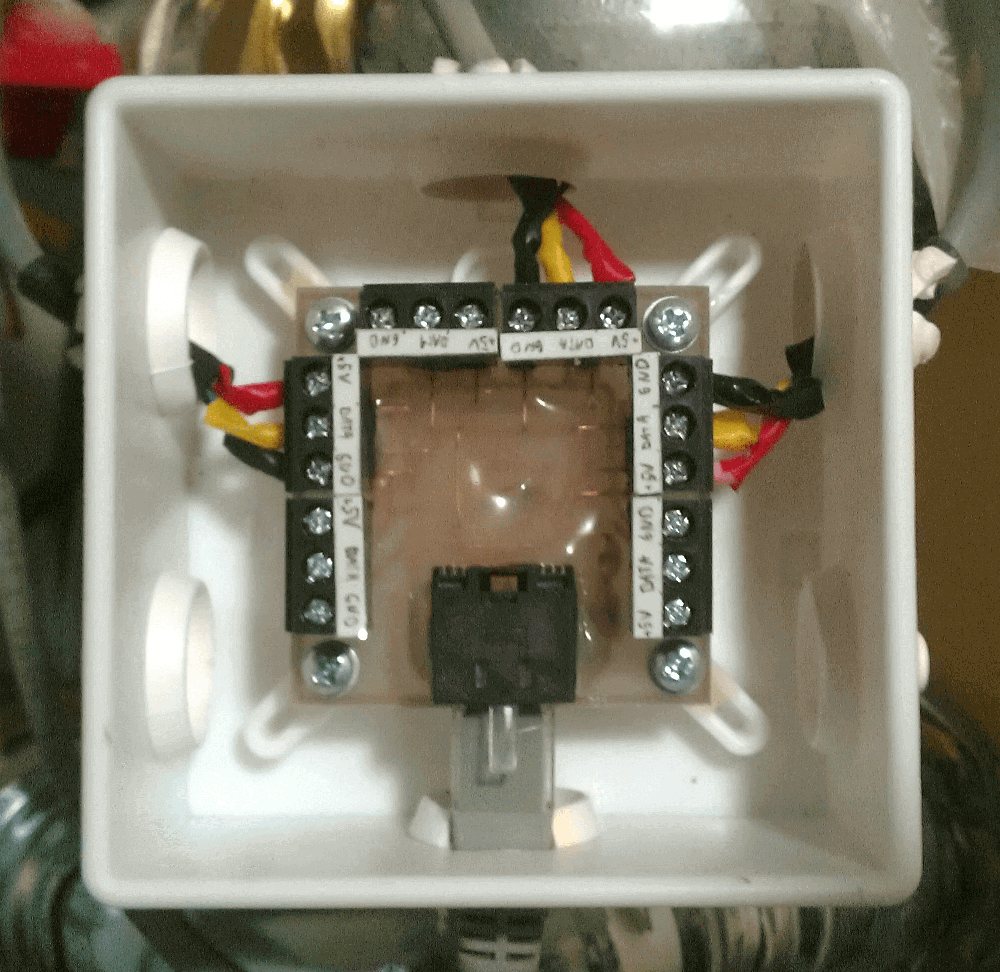
\includegraphics[width=0.95\textwidth]{images/zasobnik-otopne-vody/instalacni-krabice-cidla-u-zasobniku-otopne-vody.png}
    \caption{Horní část DPS umístěná do instalační krabice.}
    \label{fig:instalacni-krabice-cidla-u-zasobniku-otopne-vody}
\end{subfigure}%
\caption{Sdružení 1-Wire sběrnice u zásobníku otopné vody}
\end{figure}

%\begin{figure}[H]
%    \centering
%    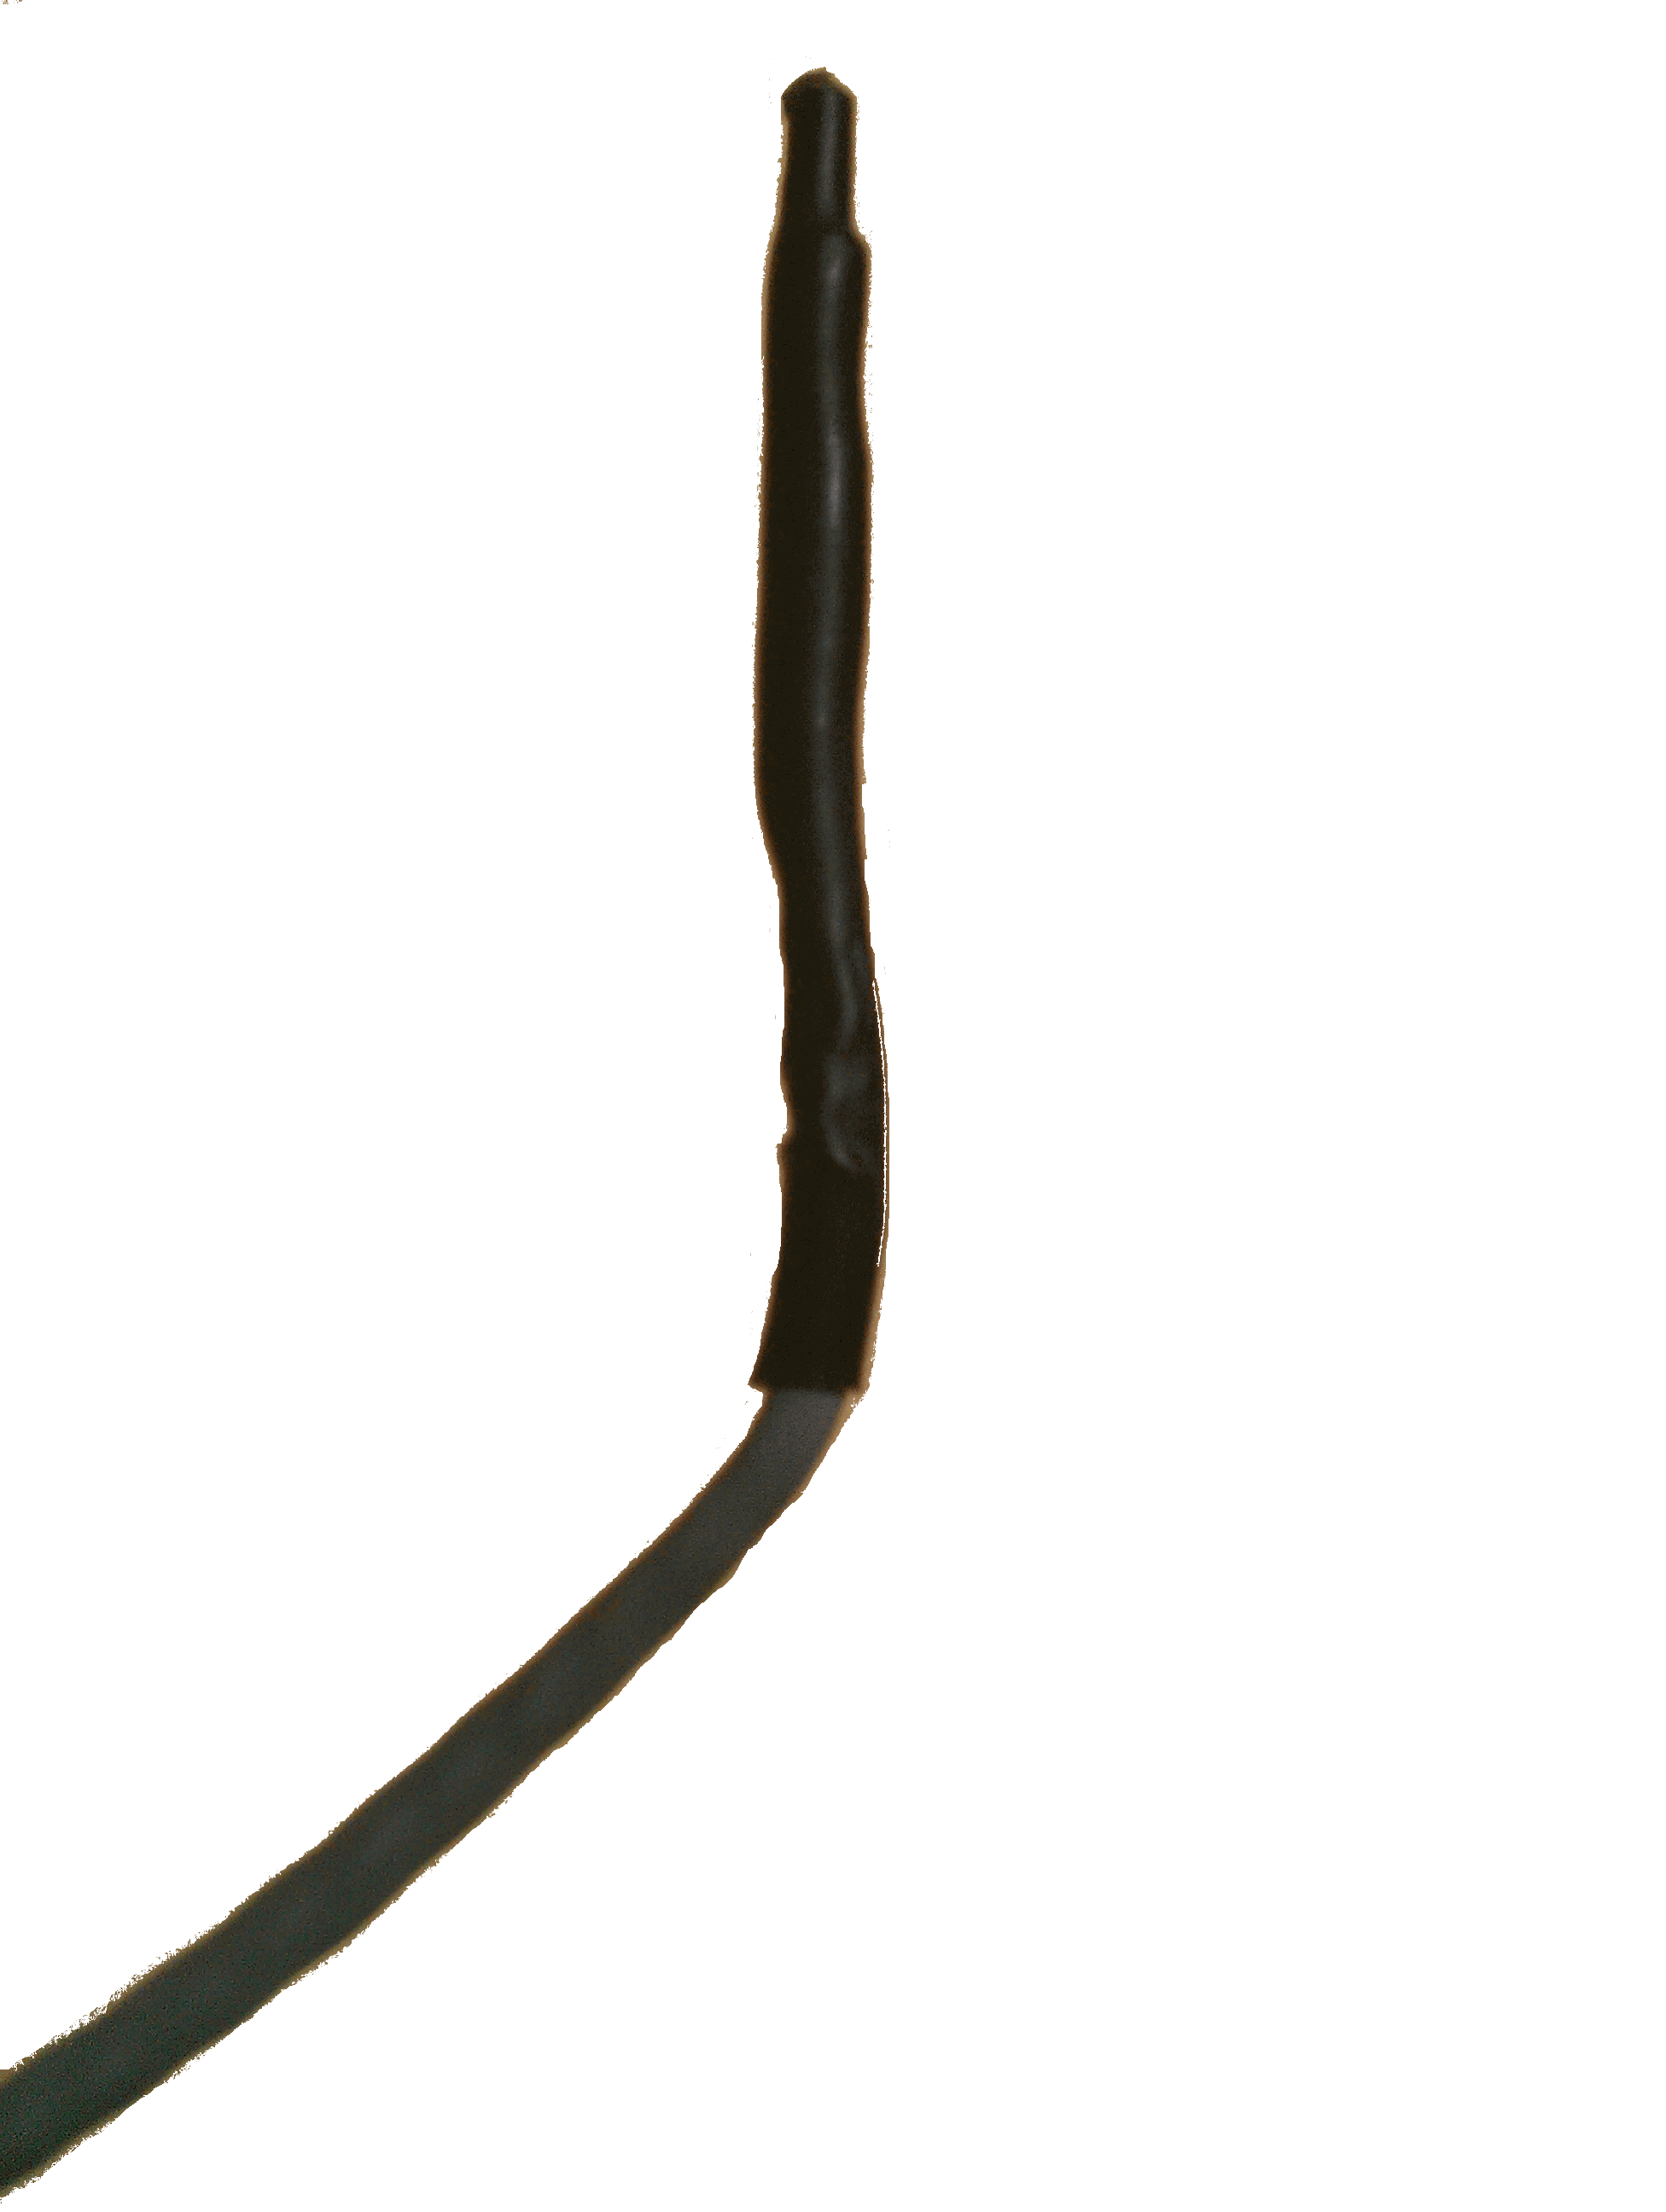
\includegraphics[width=0.4\textwidth]{images/zasobnik-otopne-vody/ds18b20-ochrana.png}
%    \caption{Teplotní senzor DS18B20 v~ochranném pouzdře.}
%    \label{fig:ds18b20-ochrana}
%\end{figure}

\begin{figure}[H]
    \centering
    \includegraphics[width=0.85\textwidth]{images/zasobnik-otopne-vody/zasobnik-otopné-vody.png}
    \caption[Zásobník otopné vody.]{Zásobník otopné vody. Červené kroužky označují místa teplotních senzorů.}
    \label{fig:zasobnik-otopné-vody}
\end{figure}